\section{Results}

To study the contribution of hard and soft processes in strangeness enhancement observed in small collision systems, results accumulated from different 
collision systems and energies for multiple strange hadrons are presented. h -- $\ks$\, and h -- $\Xi$\, correlations for minimum bias 
pp collisions at $\sqrt{s} = 5.02$ TeV and high multiplicity pp collisions $\sqrt{s} = 13$ TeV are analysed. Findings from similar studies performed 
for h -- $\Lambda$ and h -- $\phi$ correlations in p--Pb collisions at $\sqrt{s_{\mathrm{NN}}} = 5.02$ TeV are shown. 

Figure \ref{fig:pTspectra} illustrates the \pt\: spectra of $\ks$ and $\Xi$ at $\sqrt{s} = 5.02$ TeV and $\sqrt{s} = 13$ TeV. As anticipated, the 
near-side jet spectra are harder than the out-of-jet spectra, signifying different production mechanisms, with the former pertaining to hard 
particle production. The full spectra follow the shape of the out-of-jet spectra, indicating a higher relative contribution of the latter.

Calculating the $\ks$ and $\Xi$ yields per trigger particle as a function of charged particle multiplicity (Figure \ref{fig:KsXiPerTrigger}) reveals 
a stronger multiplicity dependence in the transverse to leading and full region as compared to the near-side jet region. The relative increase in 
per-trigger yield in the transverse to leading (out-of-jet) region in comparison to toward leading (near-side jet) region suggests that the relative 
contribution of soft processes increases with multiplicity.

\begin{figure}[H]
    \centering
    \begin{subfigure}{.5\textwidth}
        \centering
        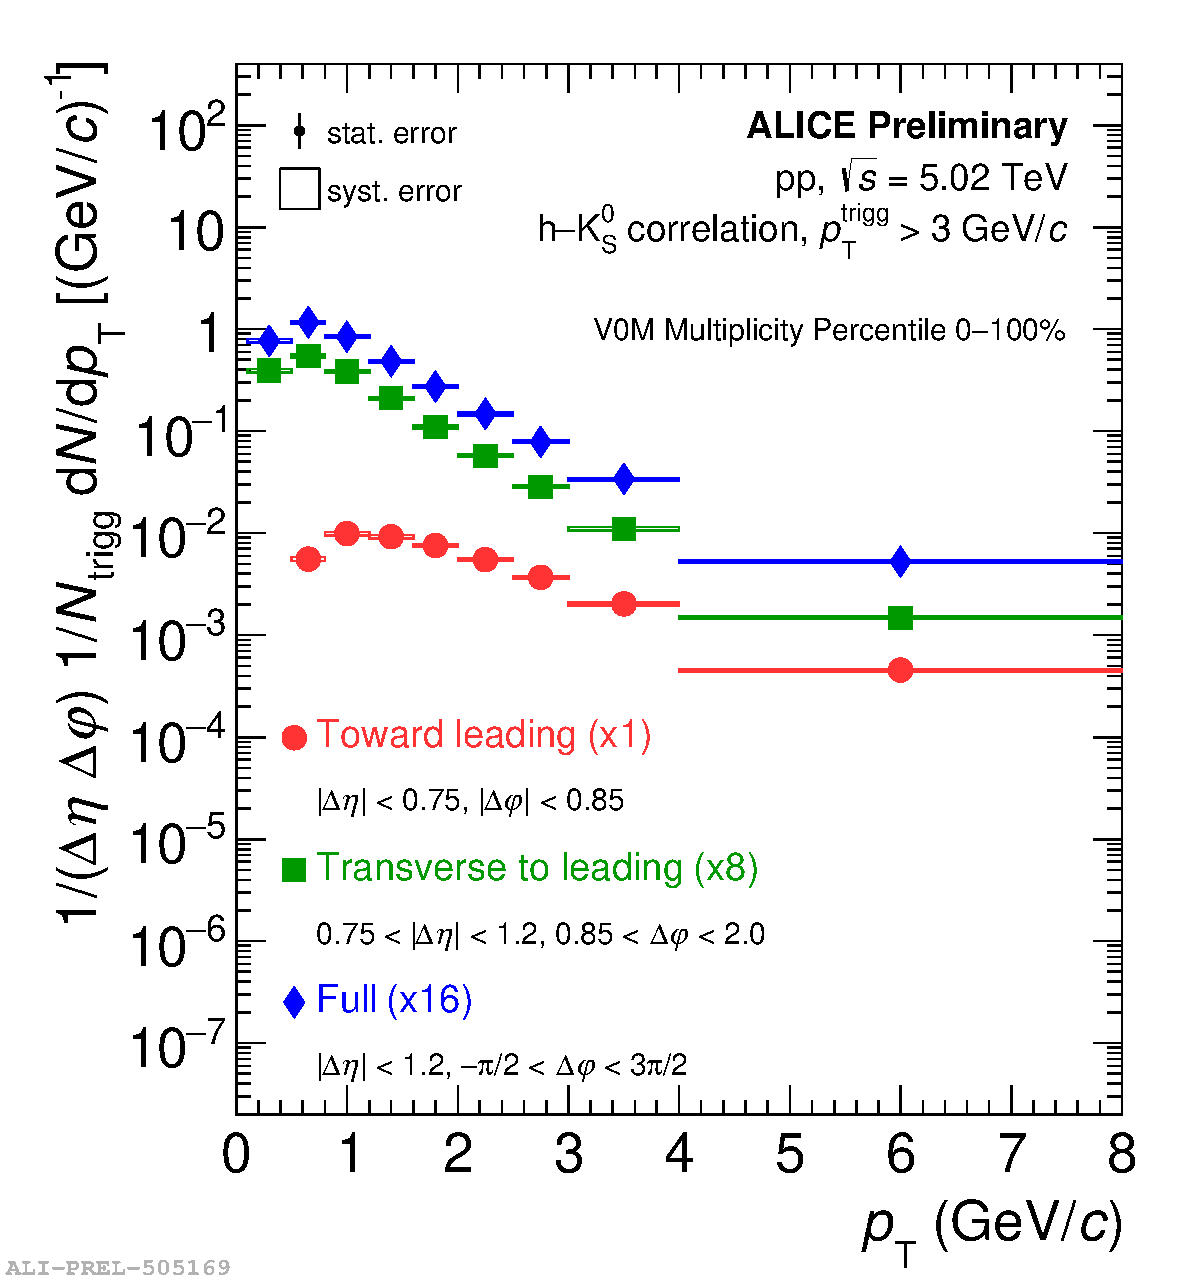
\includegraphics[width=\linewidth]{images/Ch_PtSpectraK0s_all_0.pdf}
    \end{subfigure}%
    \begin{subfigure}{.5\textwidth}
        \centering
        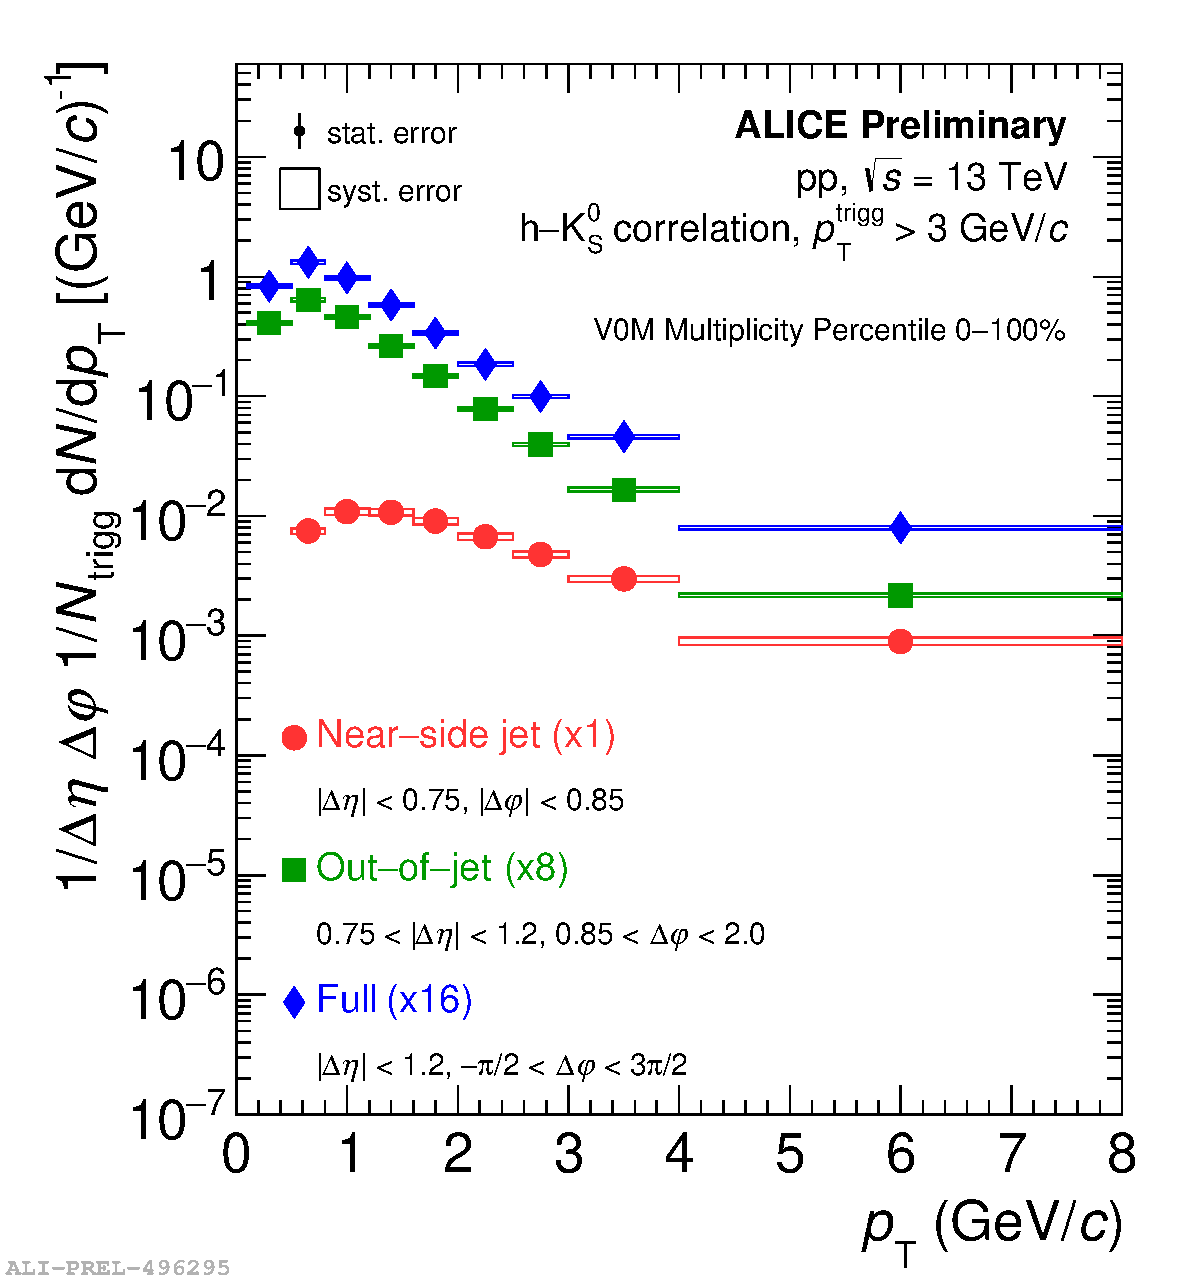
\includegraphics[width=\linewidth]{images/Ch_ptspectrak0s_all_13.pdf}
    \end{subfigure}

    \medskip
    \begin{subfigure}{.5\textwidth}
        \centering
        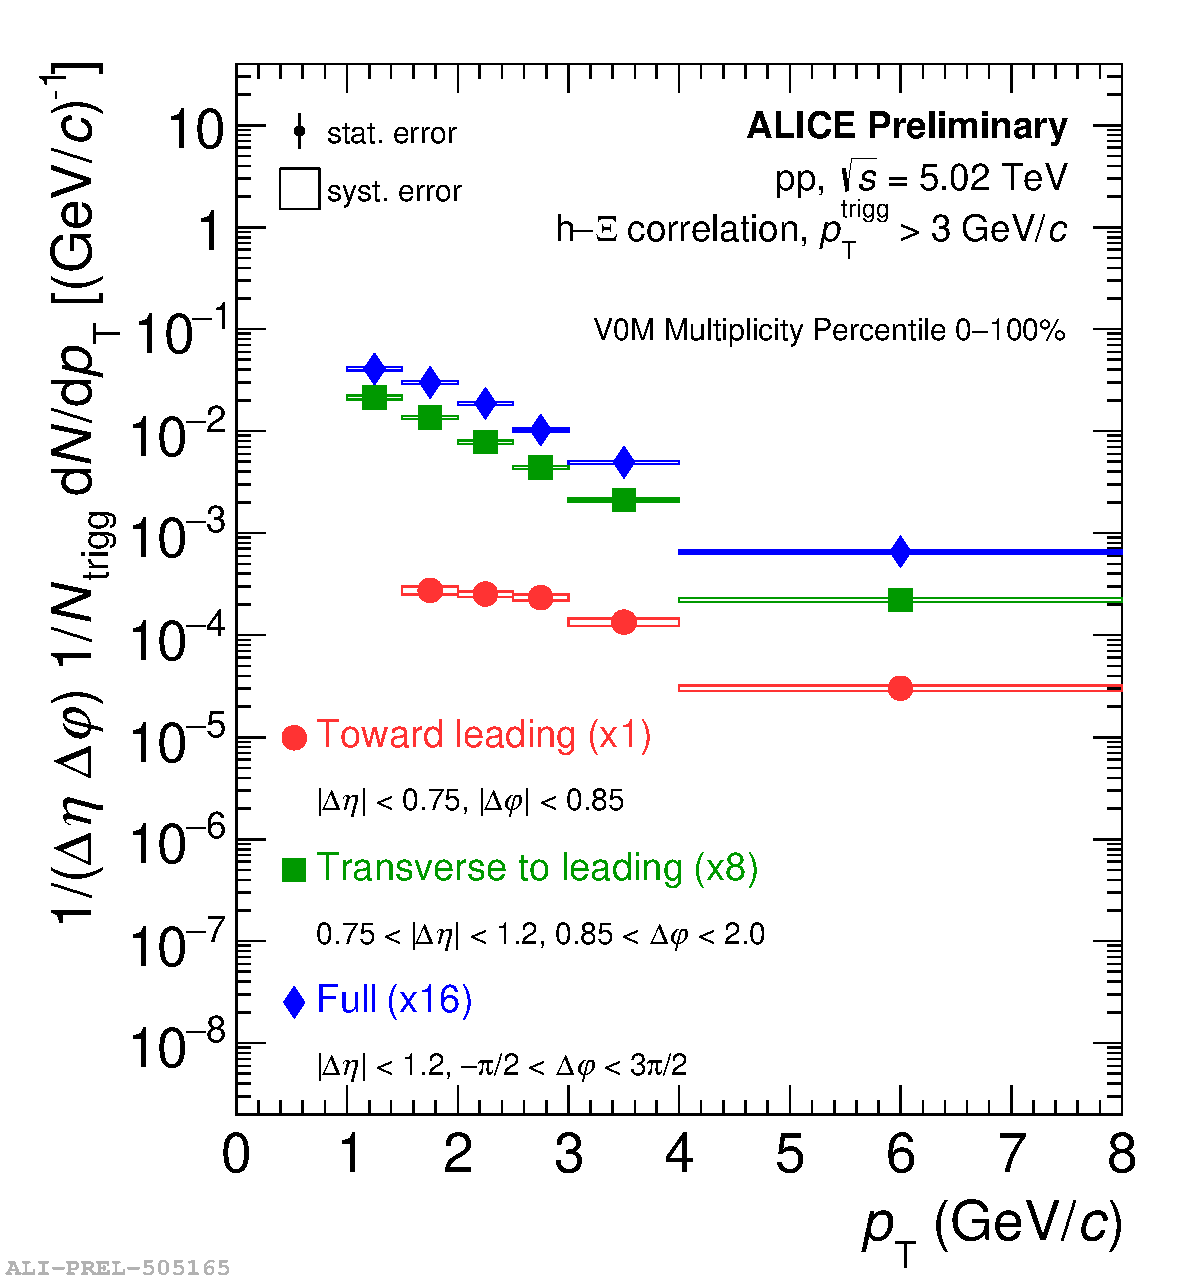
\includegraphics[width=\linewidth]{images/Ch_PtSpectraXi_all_0.pdf}
    \end{subfigure}%
    \begin{subfigure}{.5\textwidth}
        \centering
        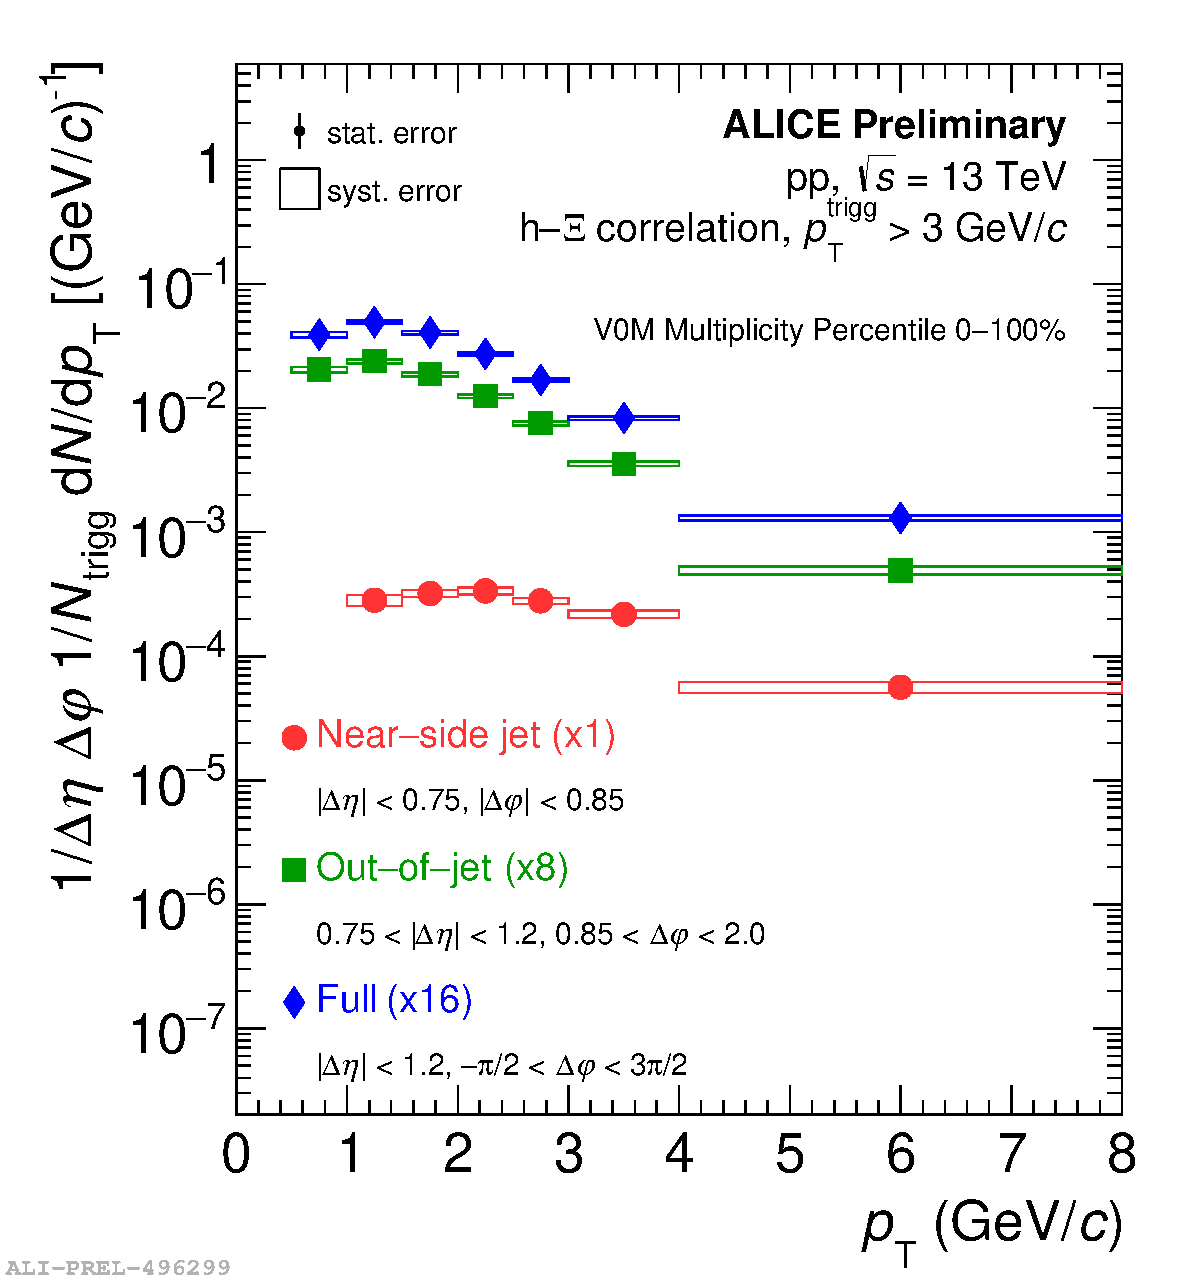
\includegraphics[width=\linewidth]{images/Ch_ptspectraxi_all_13.pdf}
    \end{subfigure}

    \caption{Toward leading (near-side jet), trasverse-to-leading (out-of-jet) and full (inclusive) transverse momentum (\pt) spectra of $\ks$ (top) 
    and $\Xi$ (bottom) for pp collisions at $\sqrt{s} = 5.02$ TeV (left) and $\sqrt{s} = 13$ TeV (right). The statistical uncertainties are represented 
    by the error bars and the total systematic uncertainty by the empty boxes.}
    \label{fig:pTspectra}
\end{figure}

To study the strangeness enhancement effect, $\Xi/\ks$ integrated yield ratio as a function of charged particle multiplicity (Figure \ref{fig:XiKsRatio}) 
is examined.
The full yield ratio increases with multiplicity owing to the larger strangeness content of $\Xi$ (|S| = 2) with respect to $\ks$ (|S| = 1).
The rise in out-of-jet and near-side jet regions seem compatible albeit the near-side ratio exhibiting larger uncertainties. The near-side jet ratio being 
smaller represents dominant contribution to the full yield ratio arising from out-of-jet processes. None of the results suggest any dependence 
on centre-of-mass energy.
\begin{figure}[H]
    \centering
    \begin{subfigure}{.5\textwidth}
        \centering
        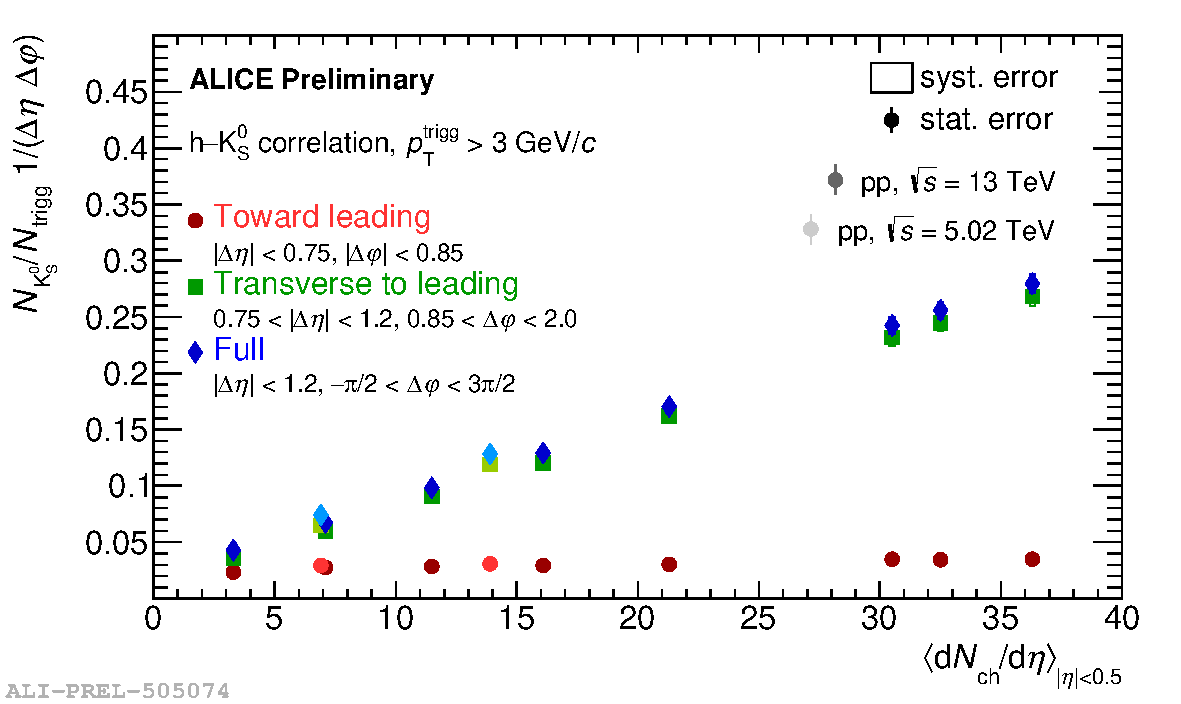
\includegraphics[width=\linewidth]{images/Ch_K0s_per_trig_yields.pdf}
    \end{subfigure}%
    \begin{subfigure}{.5\textwidth}
        \centering
        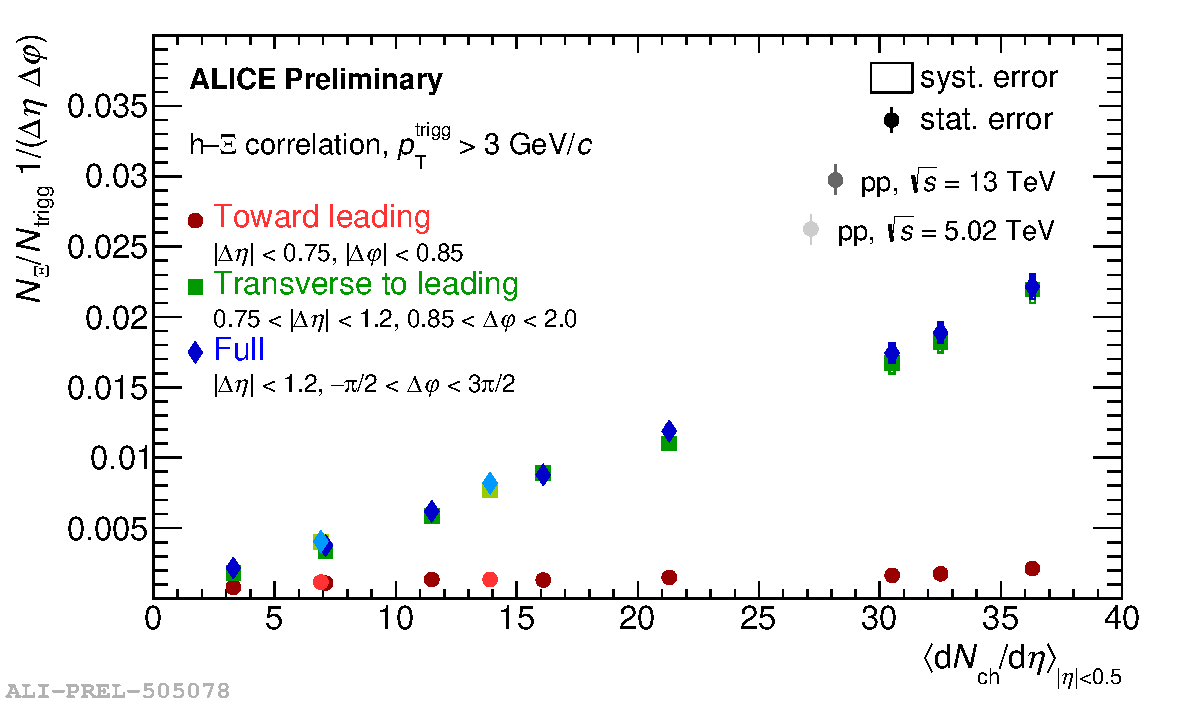
\includegraphics[width=\linewidth]{images/Ch_Xi_per_trig_yields.pdf}
    \end{subfigure}
    \caption{$\ks$ (left) and $\Xi$ (right) integrated yields ($0 < p_{\textnormal{{\sc t}, assoc}} < \infty$) per trigger particle and per unit 
    $\Delta\varphi\Delta\eta$ as a function of charged particle multiplicity at midrapidity 
    $\langle\textnormal{d}N_{\textnormal{ch}}/\textnormal{d}\eta\rangle_{|\eta|<0.5}$. The statistical uncertainties are represented 
    by the error bars and the total systematic uncertainty by the empty boxes.}
    \label{fig:KsXiPerTrigger}
\end{figure}

\begin{figure}[H]
    \centering
    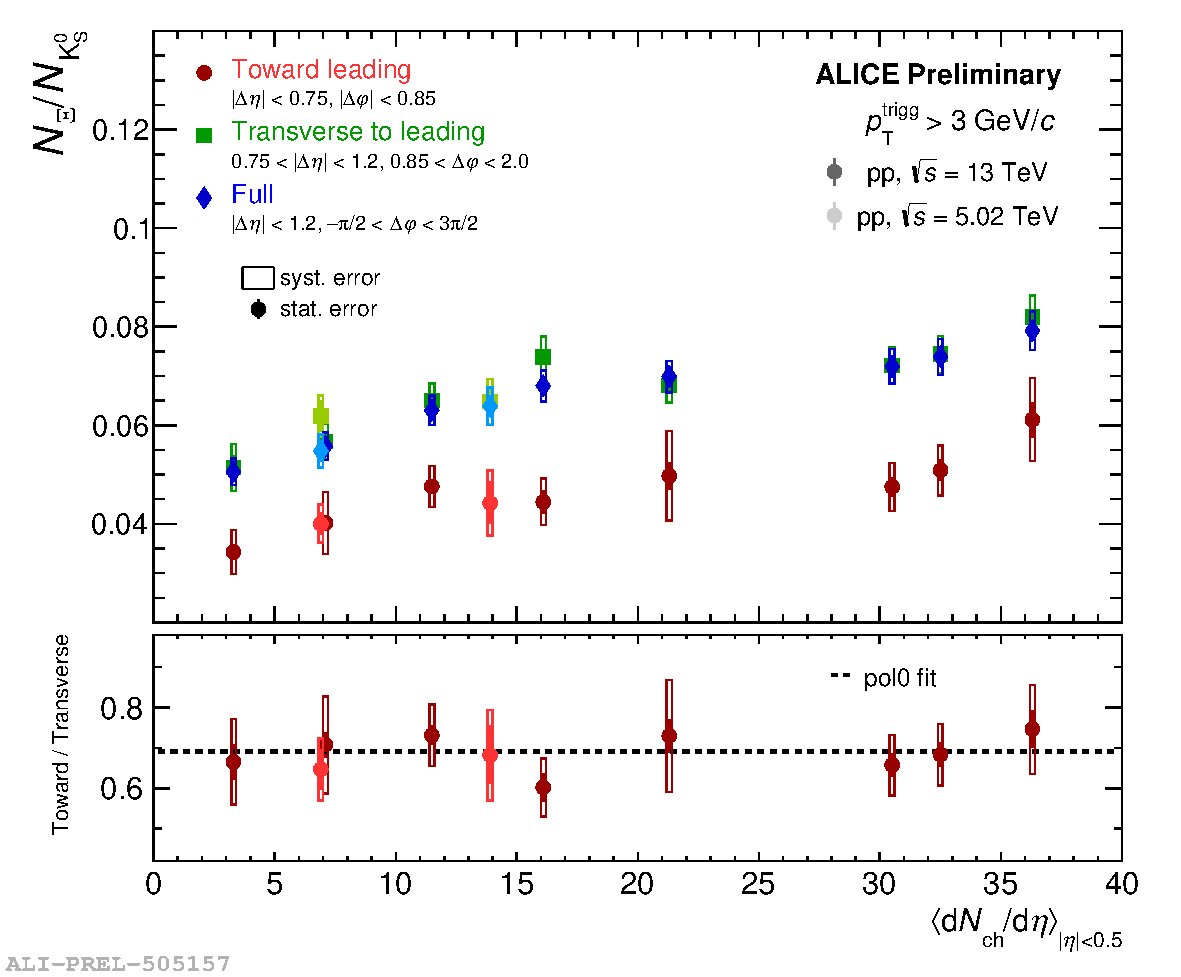
\includegraphics[width=0.75\linewidth]{images/Ch_XiK0s_Ratio.pdf}
    \\
    \caption{$\Xi/\ks$ integrated yield ratio ($0 < p_{\textnormal{{\sc t}, assoc}} < \infty$) as a function of charged particle multiplicity at 
    midrapidity $\langle\textnormal{d}N_{\textnormal{ch}}/\textnormal{d}\eta\rangle_{|\eta|<0.5}$. The statistical uncertainties are represented 
    by the error bars and the total systematic uncertainty by the empty boxes.}
    \label{fig:XiKsRatio}
\end{figure}

In case of p--Pb collisions at $\sqrt{s_{\mathrm{NN}}} = 5.02$ TeV, similar trends in strangeness enhancement can be observed (Figure \ref{fig:phiLambdaRatio}). 
For $2 < p_{\textnormal{{\sc t}, assoc}} < 4\:\mathrm{GeV}/c$, it can be seen that the yield ratios in total, out-of-jet (underlying event), away-side jet 
and near-side jet region increase as a function of multiplicity, although higher values in the underlying event region indicate a dominant 
contribution to the total yield ratio comes from soft particle production mechanisms.

\begin{figure}[H]
    \centering
    \begin{subfigure}{.5\textwidth}
        \centering
        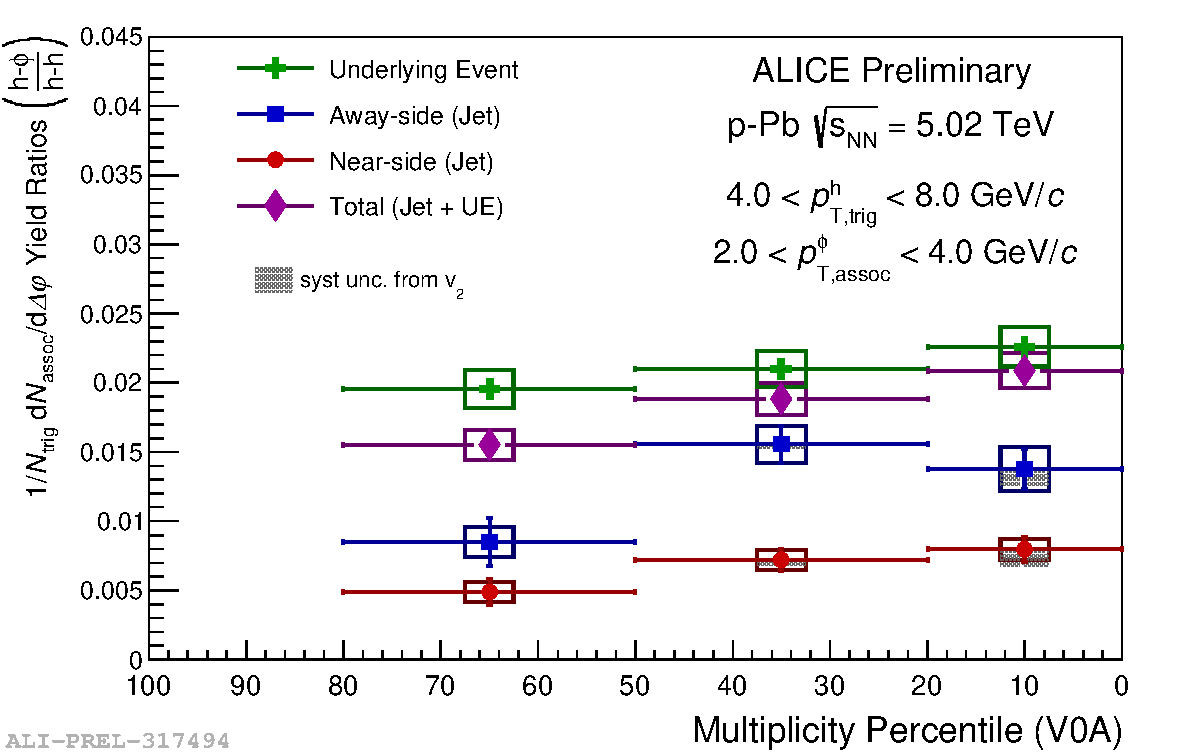
\includegraphics[width=\linewidth]{images/Jus_phi_ratio.pdf}
    \end{subfigure}%
    \begin{subfigure}{.5\textwidth}
        \centering
        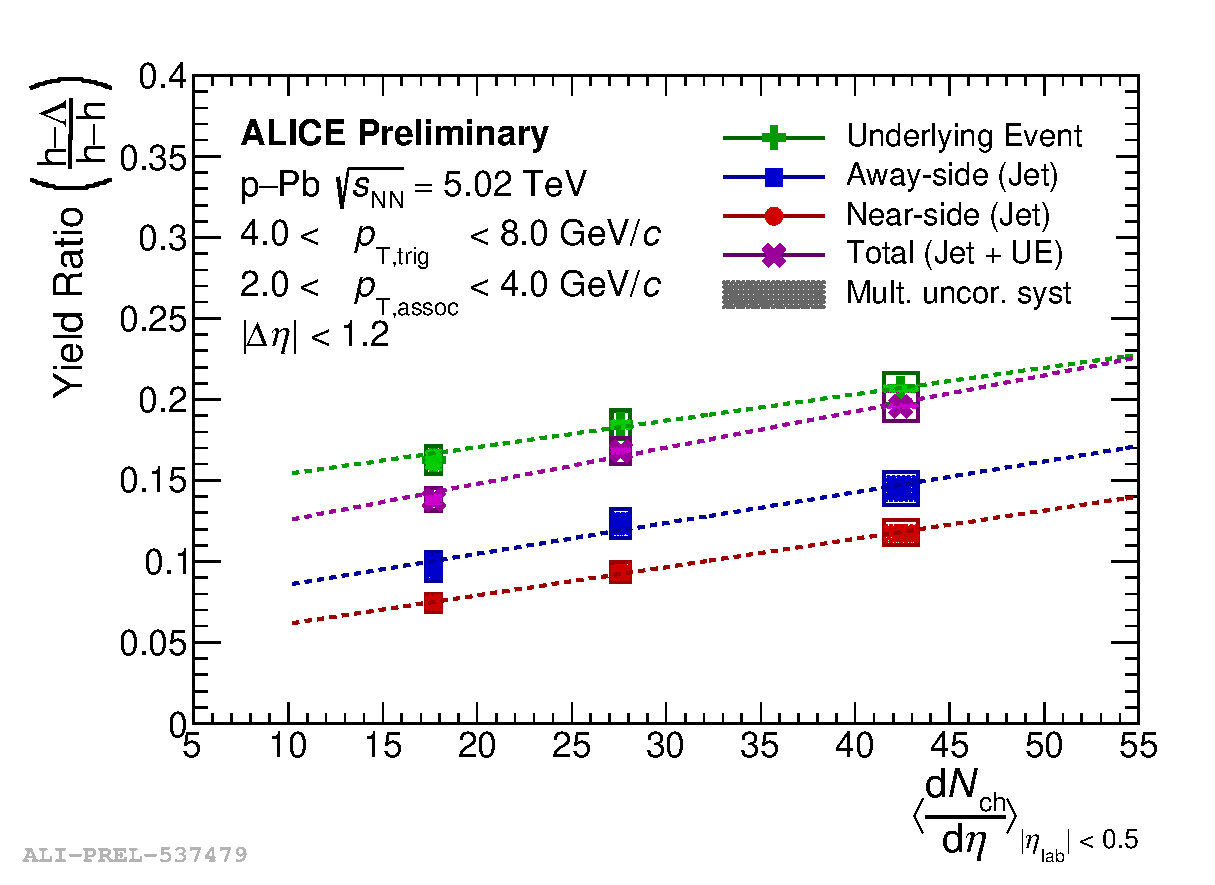
\includegraphics[width=0.9\linewidth]{images/Ry_Lambda_ratio.eps}
    \end{subfigure}
    \caption{Pair-wise per-trigger yield ratios for $\frac{\mathrm{h}-\phi}{\mathrm{h-h}}$ (left) and $\frac{\mathrm{h}-\Lambda}{\mathrm{h-h}}$ (right)
    correlated pairs as a function of charged particle multiplicity at midrapidity $\langle\textnormal{d}N_{\textnormal{ch}}/\textnormal{d}\eta\rangle_{|\eta|<0.5}$ 
    in p-Pb collisions at $\sqrt{s_{\mathrm{NN}}} = 5.02$ TeV. The statistical uncertainties are represented by the error bars and the total systematic 
    uncertainty by the empty boxes.}
    \label{fig:phiLambdaRatio}
\end{figure}


